\section{Funciones escalares}

La mayoría de los fenómenos físicos e ingenieriles dependen de múltiples variables simultáneamente: la temperatura en un sólido depende de las coordenadas $(x, y, z)$, la presión de un gas depende de la temperatura y el volumen, la resistencia de una viga depende de su geometría y del material. Para modelar estos fenómenos se introducen las funciones escalares de varias variables, que extienden el concepto de función real $f: \mathbb{R} \to \mathbb{R}$ a dominios de dimensión superior.

\subsection{Definición}

\begin{mydefinition}{Función escalar de $n$ variables}
Una función escalar de $n$ variables es una regla $f$ que asigna a cada punto $(x_1, x_2, \dots, x_n)$ en un subconjunto $D \subseteq \mathbb{R}^n$ un único número real:
\[ f: D \subseteq \mathbb{R}^n \longrightarrow \mathbb{R}, \qquad (x_1, x_2, \dots, x_n) \longmapsto f(x_1, x_2, \dots, x_n) \]
Al conjunto $D$ se le llama dominio de $f$, y al conjunto de todos los valores posibles de salida se le llama imagen o rango:
\[ \text{Im}(f) = \{f(x_1, \dots, x_n) \in \mathbb{R} : (x_1, \dots, x_n) \in D\} \]
\end{mydefinition}

\subsection{Dominio y Rango}

El dominio natural de $f$ es el conjunto de todos los puntos para los que la expresión de $f$ está matemáticamente definida. Las restricciones más frecuentes son:

\begin{itemize}
    \item \textbf{Denominadores:} $g(x,y) \neq 0$
    \item \textbf{Raíces de índice par:} $g(x,y) \geq 0$
    \item \textbf{Logaritmos:} $g(x,y) > 0$
    \item \textbf{Funciones inversas:} respetar el dominio de $\arcsin$, $\arccos$, etc.
\end{itemize}

\textbf{Ejemplo 1.} Sea $f(x,y) = \sqrt{9 - x^2 - y^2}$. La condición $9 - x^2 - y^2 \geq 0$ define el dominio:
\[ D = \{(x,y) \in \mathbb{R}^2 : x^2 + y^2 \leq 9\} \]
Este es el círculo de radio $3$ centrado en el origen. La imagen es $\text{Im}(f) = [0, 3]$: el mínimo $0$ se alcanza en la circunferencia $x^2+y^2=9$ y el máximo $3$ en el origen.

\begin{center}
\shorthandoff{>}
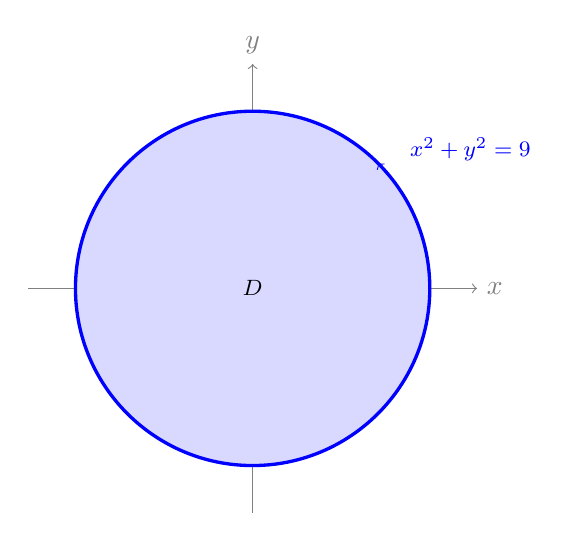
\begin{tikzpicture}[scale=0.75]
    \draw[->, gray] (-3.8,0) -- (3.8,0) node[right] {$x$};
    \draw[->, gray] (0,-3.8) -- (0,3.8) node[above] {$y$};

    \fill[blue!15] (0,0) circle (3cm);
    \draw[very thick, blue] (0,0) circle (3cm);

    \node at (0,0) [font=\footnotesize] {$D$};
    \node[above right, blue, font=\footnotesize] at (2.5, 2.0) {$x^2+y^2=9$};
    \draw[<-, blue, thin] (2.12, 2.12) -- (2.3, 1.9);
\end{tikzpicture}
\end{center}

\textbf{Ejemplo 2.} Sea $g(x,y,z) = \dfrac{\ln(1 - x^2 - y^2)}{z}$. Se necesitan dos condiciones simultáneas:
\[
    1 - x^2 - y^2 > 0 \;\Rightarrow\; x^2 + y^2 < 1
    \qquad\text{y}\qquad
    z \neq 0
\]
\[ D = \{(x,y,z) \in \mathbb{R}^3 : x^2 + y^2 < 1 \text{ y } z \neq 0\} \]

Para determinar la imagen de $f$, es útil: identificar los valores extremos en la frontera del dominio, determinar si $f$ es continua, y verificar si hay máximos o mínimos globales.

\subsection{Gráfica de funciones con dominio en $ \mathbb{R}^2 $}

Para una función de dos variables $z = f(x, y)$, la gráfica es la superficie en $\mathbb{R}^3$ formada por todos los puntos de la forma $(x, y, f(x,y))$:
\[ \text{Graf}(f) = \bigl\{(x,\, y,\, f(x,y)) \in \mathbb{R}^3 : (x,y) \in D\bigr\} \]
Cada punto del plano $xy$ se eleva o hunde según el valor que $f$ le asigna.

\textbf{Ejemplo 1.} Paraboloide elíptico: $f(x,y) = x^2 + y^2$

Esta superficie tiene un mínimo global en el origen $(0,0,0)$ y crece sin límite al alejarse. En cualquier plano vertical que pase por el eje $z$, la sección es una parábola.

\begin{center}
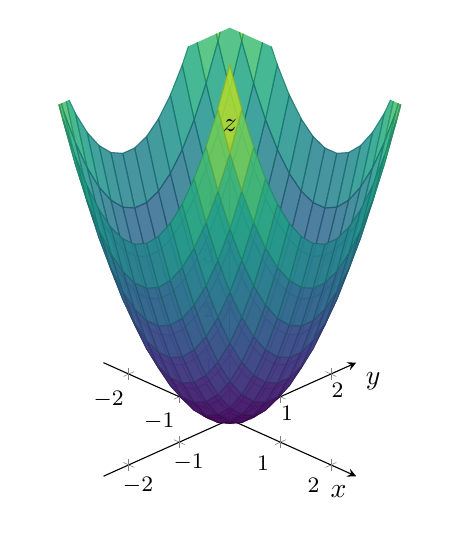
\begin{tikzpicture}
\begin{axis}[
    view={45}{30},
    axis lines=center,
    xlabel={$x$}, ylabel={$y$}, zlabel={$z$},
    xlabel style={anchor=north east},
    ylabel style={anchor=north west},
    zlabel style={anchor=south},
    xmin=-2.5, xmax=2.5,
    ymin=-2.5, ymax=2.5,
    zmin=0,    zmax=5,
    xtick={-2,-1,0,1,2}, ytick={-2,-1,0,1,2}, ztick={1,2,3,4},
    tick label style={font=\footnotesize},
    width=8cm, height=8cm,
    colormap/viridis,
]
    \addplot3[
        surf, opacity=0.85,
        domain=-2:2, domain y=-2:2,
        samples=18,
    ] {x^2 + y^2};
\end{axis}
\end{tikzpicture}
\end{center}

\textbf{Ejemplo 2.} Silla de montar (paraboloide hiperbólico): $f(x,y) = x^2 - y^2$

Esta superficie sube como una parábola en la dirección $x$ y baja como una parábola en la dirección $y$. El punto $(0,0,0)$ es un punto de silla: no es ni máximo ni mínimo local.

\begin{center}
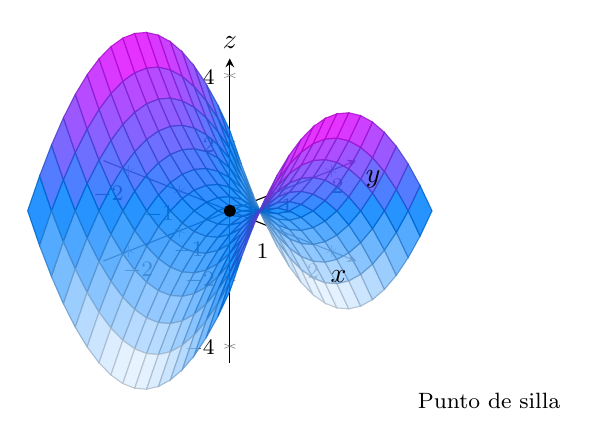
\begin{tikzpicture}
\begin{axis}[
    view={45}{25},
    axis lines=center,
    xlabel={$x$}, ylabel={$y$}, zlabel={$z$},
    xlabel style={anchor=north east},
    ylabel style={anchor=north west},
    zlabel style={anchor=south},
    xmin=-2.5, xmax=2.5,
    ymin=-2.5, ymax=2.5,
    zmin=-4.5, zmax=4.5,
    xtick={-2,-1,0,1,2}, ytick={-2,-1,0,1,2},
    tick label style={font=\footnotesize},
    width=8cm, height=8cm,
    colormap/cool,
]
    \addplot3[
        surf, opacity=0.85,
        domain=-2:2, domain y=-2:2,
        samples=18,
    ] {x^2 - y^2};
    \addplot3[mark=*, mark size=2pt, black] coordinates {(0,0,0)};
\end{axis}
\node[font=\footnotesize] at (6.5, 0.8) {Punto de silla};
\end{tikzpicture}
\end{center}

\subsection{Curvas de nivel de funciones con dominio en $\mathbb{R}^2$}

Visualizar una superficie en papel es limitado. Una alternativa es proyectar sobre el plano $xy$ las intersecciones de la superficie con planos horizontales $z = c$.

\begin{mydefinition}{Curvas de nivel}
La curva de nivel de $f(x,y)$ para el valor $c \in \mathbb{R}$ es el conjunto:
\[ C_c = \{(x,y) \in D : f(x,y) = c\} \]
La colección de curvas de nivel para distintos valores de $c$ se llama mapa de contorno de $f$. Es la representación que usan los mapas topográficos: cada curva une puntos con la misma altitud.
\end{mydefinition}

La curva de nivel $C_c$ es la proyección sobre el plano $xy$ de la intersección de la superficie $z = f(x,y)$ con el plano horizontal $z = c$. Curvas de nivel muy juntas indican que la función cambia rápidamente; curvas muy separadas indican cambio lento.

\textbf{Ejemplo 1.} Curvas de nivel del paraboloide: $f(x,y) = x^2 + y^2$

La ecuación $x^2 + y^2 = c$ define círculos de radio $\sqrt{c}$ (solo para $c > 0$). Para $c = 0$ el único punto es el origen.

\begin{center}
\shorthandoff{>}
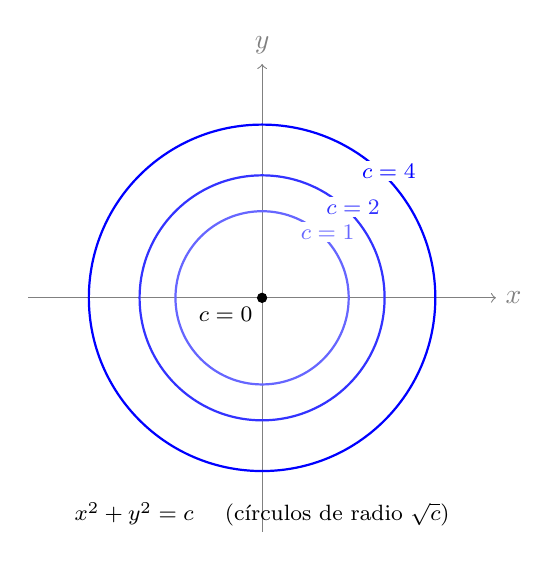
\begin{tikzpicture}[scale=1.1]
    \draw[->, gray] (-2.7,0) -- (2.7,0) node[right] {$x$};
    \draw[->, gray] (0,-2.7) -- (0,2.7) node[above] {$y$};

    % Curvas de nivel: circulos de radio sqrt(c)
    \foreach \c/\col in {1/blue!60, 2/blue!80, 4/blue}{
        \pgfmathsetmacro{\rad}{sqrt(\c)}
        \draw[\col, thick] (0,0) circle (\rad cm);
        \pgfmathsetmacro{\labelx}{\rad * 0.707}
        \node[\col, font=\footnotesize, fill=white, inner sep=1pt]
            at (\labelx+0.05, \labelx+0.05) {$c=\c$};
    }

    \filldraw[black] (0,0) circle (1.5pt) node[below left, font=\footnotesize] {$c=0$};

    \node[font=\footnotesize, align=center] at (0,-2.5)
        {$x^2+y^2 = c$ \quad (círculos de radio $\sqrt{c}$)};
\end{tikzpicture}
\end{center}

Nótese que las curvas están más separadas en el origen (la función sube lentamente) y más juntas hacia afuera (la función sube más rápido). Esto refleja que la pendiente de la parábola es mayor lejos del vértice.

\textbf{Ejemplo 2.} Curvas de nivel de la silla de montar: $f(x,y) = x^2 - y^2$

La ecuación $x^2 - y^2 = c$ define hipérbolas (para $c \neq 0$) o dos rectas cruzadas (para $c = 0$).

\begin{center}
\shorthandoff{>}
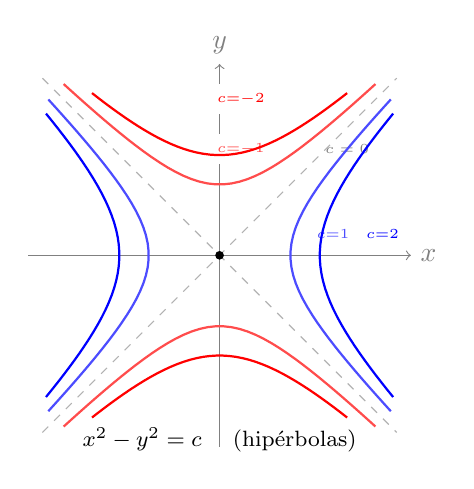
\begin{tikzpicture}[scale=0.9]
    \draw[->, gray] (-2.7,0) -- (2.7,0) node[right] {$x$};
    \draw[->, gray] (0,-2.7) -- (0,2.7) node[above] {$y$};

    % c=0: asíntotas y=x, y=-x
    \draw[gray!60, dashed] (-2.5,-2.5) -- (2.5,2.5);
    \draw[gray!60, dashed] (-2.5,2.5) -- (2.5,-2.5);
    \node[gray, font=\tiny] at (1.8, 1.5) {$c=0$};

    % c=1: hiperbola x^2 - y^2 = 1 (abre en x), rama derecha e izq
    \draw[blue!70, thick, domain=-2.2:2.2, samples=40]
        plot ({sqrt(1+\x*\x)}, {\x});
    \draw[blue!70, thick, domain=-2.2:2.2, samples=40]
        plot ({-sqrt(1+\x*\x)}, {\x});
    \node[blue!70, font=\tiny, fill=white] at (1.6, 0.3) {$c{=}1$};

    % c=2: hiperbola x^2 - y^2 = 2
    \draw[blue, thick, domain=-2.0:2.0, samples=40]
        plot ({sqrt(2+\x*\x)}, {\x});
    \draw[blue, thick, domain=-2.0:2.0, samples=40]
        plot ({-sqrt(2+\x*\x)}, {\x});
    \node[blue, font=\tiny, fill=white] at (2.3, 0.3) {$c{=}2$};

    % c=-1: hiperbola y^2 - x^2 = 1 (abre en y)
    \draw[red!70, thick, domain=-2.2:2.2, samples=40]
        plot ({\x}, {sqrt(1+\x*\x)});
    \draw[red!70, thick, domain=-2.2:2.2, samples=40]
        plot ({\x}, {-sqrt(1+\x*\x)});
    \node[red!70, font=\tiny, fill=white] at (0.3, 1.5) {$c{=}{-}1$};

    % c=-2
    \draw[red, thick, domain=-1.8:1.8, samples=40]
        plot ({\x}, {sqrt(2+\x*\x)});
    \draw[red, thick, domain=-1.8:1.8, samples=40]
        plot ({\x}, {-sqrt(2+\x*\x)});
    \node[red, font=\tiny, fill=white] at (0.3, 2.2) {$c{=}{-}2$};

    \filldraw[black] (0,0) circle (1.5pt);
    \node[font=\footnotesize, align=center] at (0,-2.6) {$x^2 - y^2 = c$ \quad (hipérbolas)};
\end{tikzpicture}
\end{center}

Las hipérbolas azules ($c > 0$) abren en la dirección $x$ y las rojas ($c < 0$) abren en la dirección $y$, reflejando que la función sube en $x$ y baja en $y$.

\subsection{Superficies de nivel de funciones con dominio en $\mathbb{R}^3$}

Para una función de tres variables $w = f(x, y, z)$, la gráfica sería un objeto en $\mathbb{R}^4$, imposible de visualizar directamente. El análogo de las curvas de nivel son las superficies de nivel.

\begin{mydefinition}{Superficie de nivel}
La superficie de nivel de $f(x,y,z)$ para el valor $c \in \mathbb{R}$ es el conjunto:
\[ S_c = \{(x,y,z) \in D : f(x,y,z) = c\} \]
Cada superficie de nivel es un subconjunto del espacio $\mathbb{R}^3$ y representa todos los puntos donde $f$ toma el mismo valor $c$.
\end{mydefinition}

\textbf{Ejemplo 1.} $f(x,y,z) = x^2 + y^2 + z^2$

Las superficies de nivel son $x^2 + y^2 + z^2 = c$, que son esferas concéntricas de radio $\sqrt{c}$ centradas en el origen (para $c > 0$).

\begin{center}
\shorthandoff{>}
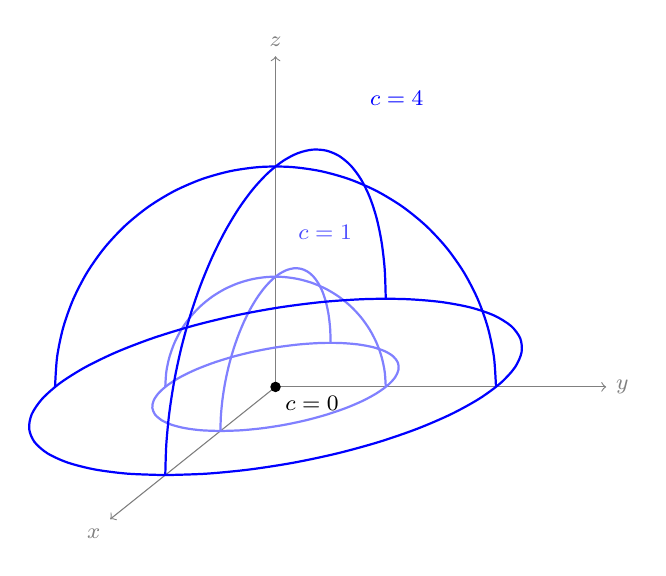
\begin{tikzpicture}[x={(-0.5cm,-0.4cm)}, y={(1cm,0cm)}, z={(0cm,1cm)}, scale=1.4]
    \draw[->, gray] (0,0,0) -- (3,0,0) node[below left, font=\footnotesize] {$x$};
    \draw[->, gray] (0,0,0) -- (0,3,0) node[right, font=\footnotesize] {$y$};
    \draw[->, gray] (0,0,0) -- (0,0,3) node[above, font=\footnotesize] {$z$};

    % Esfera c=1 (radio 1): arcos representativos
    \draw[blue!50, thick, variable=\t, domain=0:360, samples=36, smooth]
        plot ({cos(\t)}, {sin(\t)}, 0);
    \draw[blue!50, thick, variable=\t, domain=0:180, samples=24, smooth]
        plot ({cos(\t)}, 0, {sin(\t)});
    \draw[blue!50, thick, variable=\t, domain=0:180, samples=24, smooth]
        plot (0, {cos(\t)}, {sin(\t)});
    \node[blue!70, font=\footnotesize] at (-1.5, -0.3, 0.8) {$c=1$};

    % Esfera c=4 (radio 2): arcos representativos
    \draw[blue, thick, variable=\t, domain=0:360, samples=36, smooth]
        plot ({2*cos(\t)}, {2*sin(\t)}, 0);
    \draw[blue, thick, variable=\t, domain=0:180, samples=24, smooth]
        plot ({2*cos(\t)}, 0, {2*sin(\t)});
    \draw[blue, thick, variable=\t, domain=0:180, samples=24, smooth]
        plot (0, {2*cos(\t)}, {2*sin(\t)});
    \node[blue, font=\footnotesize] at (-2.8, -0.3, 1.5) {$c=4$};

    \filldraw[black] (0,0,0) circle (1.2pt) node[below right, font=\footnotesize] {$c=0$};
\end{tikzpicture}
\end{center}

\textbf{Ejemplo 2.} $g(x,y,z) = x^2 + y^2$

Las superficies de nivel de $g$ son $x^2 + y^2 = c$, que son cilindros circulares de radio $\sqrt{c}$ con eje en la dirección $z$. La función no depende de $z$, de modo que para cada nivel $c$ hay una familia de circunferencias apiladas verticalmente.

\subsection{Ejercicios}

\begin{enumerate}
    \item Determinar el dominio natural de cada función escalar e indicar a qué conjunto geométrico corresponde en $\mathbb{R}^2$ o $\mathbb{R}^3$:
\begin{enumerate}
    \item $f(x,y) = \sqrt{16 - x^2 - 4y^2}$
    \item $g(x,y) = \ln(y - x^2)$
    \item $h(x,y) = \dfrac{1}{\sqrt{x^2 + y^2 - 1}}$
\end{enumerate}
    \item Determinar el dominio natural de cada función de tres variables y describir geométricamente la región en $\mathbb{R}^3$:
\begin{enumerate}
    \item $f(x,y,z) = \sqrt{4 - x^2 - y^2 - z^2}$
    \item $g(x,y,z) = \dfrac{\arcsin(z)}{\sqrt{x^2 + y^2}}$
\end{enumerate}
    \item Para la función $f(x,y) = \sqrt{x + y} + \sqrt{4 - x^2}$:
\begin{enumerate}
    \item Encontrar el dominio natural $D$ e identificarlo geométricamente (trazar o describir la región).
    \item Determinar la imagen de $f$.
    \item Verificar que el punto $(1, 0)$ pertenece a $D$ y calcular $f(1, 0)$.
\end{enumerate}
    \item Identificar y nombrar la superficie definida por cada función $z = f(x,y)$, describiendo su forma geométrica (paraboloide, silla de montar, plano, cono, cilindro, etc.) y señalando características clave como vértice, eje de simetría o punto de silla:
\begin{enumerate}
    \item $f(x,y) = 3x - 2y + 5$
    \item $f(x,y) = x^2 + 4y^2$
    \item $f(x,y) = \sqrt{x^2 + y^2}$
    \item $f(x,y) = 4 - x^2 - y^2$
\end{enumerate}
    \item Para $f(x,y) = x^2 + 4y^2$, trazar las curvas de nivel correspondientes a $c = 0, 1, 4, 9$ en el plano $xy$.
\begin{enumerate}
    \item Determinar la forma geométrica de cada curva de nivel e indicar sus semiejes.
    \item ¿Qué ocurre con el espaciado entre curvas de nivel conforme $c$ aumenta? ¿Qué dice esto sobre la ``pendiente'' de la superficie?
    \item ¿Para qué valores de $c$ existen curvas de nivel? ¿Cuál es la imagen de $f$?
\end{enumerate}
    \item Trazar las curvas de nivel de $f(x,y) = xy$ para $c = -2, -1, 0, 1, 2$ e identificar su forma.
\begin{enumerate}
    \item Mostrar que para $c \neq 0$ cada curva de nivel es una hipérbola y determinar sus asíntotas.
    \item ¿Qué ocurre con la curva de nivel $c = 0$? Describir el conjunto $\{(x,y): xy = 0\}$.
    \item Usando el mapa de contorno, describir el comportamiento de $f$ cerca del origen: ¿tiene máximo, mínimo o punto de silla?
\end{enumerate}
    \item Se dan las ecuaciones de las curvas de nivel de una función $f(x,y)$. En cada caso, identificar una posible expresión para $f(x,y)$ justificando la elección:
\begin{enumerate}
    \item Las curvas de nivel son rectas paralelas de la forma $2x - y = c$.
    \item Las curvas de nivel son circunferencias centradas en $(1, 2)$.
    \item Las curvas de nivel son parábolas de la forma $y = x^2 + c$.
    \item Las curvas de nivel para $c > 0$ son elipses, y no existen para $c < 0$.
\end{enumerate}
    \item Para cada función de tres variables, identificar y describir geométricamente sus superficies de nivel para $c = 1, 4, 9$:
\begin{enumerate}
    \item $f(x,y,z) = x^2 + y^2$ \quad (¿depende de $z$?)
    \item $g(x,y,z) = x^2 + y^2 - z^2$
    \item $h(x,y,z) = 2x + 3y - z$
\end{enumerate}
Para el inciso (b), distinguir los casos $c > 0$, $c = 0$ y $c < 0$.
    \item Un mapa topográfico de una montaña muestra curvas de nivel equiespaciadas en altura ($\Delta z = 100$ m) a distancias horizontales que varían de un punto a otro. En la zona $A$ las curvas están muy juntas; en la zona $B$ están muy separadas.
\begin{enumerate}
    \item ¿En cuál zona es más pronunciada la pendiente del terreno? Justificar usando la interpretación de las curvas de nivel.
    \item Si $z = f(x,y)$ modela la altitud, y en la zona $A$ una curva de nivel $c=500$ m y la siguiente $c=600$ m están separadas apenas $50$ m horizontalmente, mientras que en la zona $B$ están separadas $500$ m, estimar la ``pendiente media'' en cada zona como $\Delta z / \Delta d$.
    \item Proponer una función $f(x,y)$ sencilla cuyas curvas de nivel tengan la forma general de un volcán (alto en el centro, nivel descendente hacia afuera).
\end{enumerate}
    \item La distribución de temperatura en una placa metálica cuadrada $[-2,2]\times[-2,2]$ está modelada por:
\[ T(x,y) = 100 - 10x^2 - 20y^2 \quad (^\circ\text{C}) \]
\begin{enumerate}
    \item Encontrar el dominio y la imagen de $T$ sobre la placa.
    \item Calcular la temperatura en los puntos $(0,0)$, $(1,1)$ y $(2, 0)$.
    \item Trazar las curvas de nivel (isotermas) para $T = 100, 80, 60, 40, 20$ °C. ¿Qué forma tienen? ¿Cuáles de ellas intersectan la placa?
    \item Determinar el conjunto de puntos de la placa donde la temperatura es de exactamente $70$ °C e identificarlo geométricamente.
    \item Una partícula se mueve sobre la placa siguiendo la trayectoria $\vec{r}(t) = (t, t^2 - 1)$ para $t \in [-1, 1]$. Calcular $T(x(t), y(t))$ a lo largo de esta trayectoria y encontrar el punto de temperatura máxima.
\end{enumerate}
\end{enumerate}